\documentclass[]{article}
\usepackage{amsmath}
\usepackage{amsthm}
\usepackage{amssymb}
\usepackage{authblk}
\usepackage{mathtools}
\usepackage{makecell}
\usepackage{physics}
\usepackage{hyperref}
%\usepackage{bbm} % JK have trouble installing this
\usepackage{multirow}
\usepackage[table]{xcolor}
\usepackage{booktabs}
\usepackage[utf8]{inputenc}
\usepackage{adjustbox}
\usepackage{caption}
\usepackage{rotating}
% JK: personal preference: join paper.includes + paper.definitions
%     and write any definitions which rely on the package
%     immediately after loading the package so you can see dependencies.

% JK: personal formatting preference:
\usepackage[margin=3cm]{geometry}
\DeclarePairedDelimiter{\floor}{\lfloor}{\rfloor}
\DeclarePairedDelimiter{\ceil}{\lceil}{\rceil}
%\newcommand{\ind}{\mathbbm{1}}
\usepackage{bm}\newcommand{\ind}{\bm{1}}
\DeclareUnicodeCharacter{2713}{\checkmark}
\setlength{\parskip}{1em}

\title{A flexible integer linear programming formulation for scheduling
	clinician on-call service in hospitals}

\author[a, b]{David Landsman}
\author[a]{Huiting Ma}
\author[a]{Jesse Knight}
\author[c]{Kevin Gough}
\author[a, c, d, e]{Sharmistha Mishra}

\renewcommand\Affilfont{\itshape\small}
\affil[a]{MAP Centre for Urban Health Solutions, Unity Health Toronto, Toronto,
	ON, Canada}
\affil[b]{Department of Computer Science, University of Toronto, Toronto, ON,
	Canada}
\affil[c]{Department of Medicine, Division of Infectious Disease, St.\ Michael's
	Hospital, University of Toronto, Toronto, ON, Canada}
\affil[d]{Institute of Health Policy, Management and Evaluation, Dalla Lana
	School of Public Health, University of Toronto, Toronto, ON, Canada}
\affil[e]{Institute of Medical Sciences, University of Toronto, Toronto, ON,
	Canada}

\begin{document}
	\maketitle
	
	\begin{abstract}
		Scheduling of personnel in a hospital environment is vital to improving the service provided to patients and balancing the workload assigned to clinicians. Many approaches have been tried and successfully applied to generate efficient schedules in such settings. However, due to the computational complexity of the scheduling problem in general, most approaches resort to heuristics to find a non-optimal solution in a reasonable amount of time. We designed an integer linear programming formulation to find an optimal schedule in a clinical division of a hospital. Our formulation mitigates computational complexity issues by maintaining a minimal set of constraints, yet still provides the flexibility necessary to adapt it to a variety of clinical divisions. \\

We then conducted a case study for our approach using data from the Infectious Diseases division at St. Michael's Hospital in Toronto, Canada. We analyzed and compared the results of our approach to manually-created schedules at the hospital, and found improved adherence to departmental constraints and clinician preferences. We used simulated data to examine the sensitivity of the runtime of our linear program for various parameters and observed reassuring results, signifying the practicality and generazability of our approach in different real-world scenarios.
	\end{abstract}
	
	\section{Introduction}\label{sec:introduction}
	On-call schedules for a fixed number of health-care providers are central to the efficient running of hospitals. Hospital departments provide services where patient needs, and thus the system's demands, often exceed the available supply. For example, it is important that a hospital department allocates its resources, such as the availability of a finite number of clinicians, optimally, to ensure the best possible service for its patients. Carefully allocated on-call schedules are meant to simultaneously ensure sufficient resources are provided to patients while not overworking clinicians to prevent costly mistakes [ref]. It is common practice for on-call schedules to be created manually. Yet manually-created schedules are prone to errors and potential for biases [ref]. First, when there is a large number of clinicians in a single department, or the constraints that need to be satisfied by the department are very complex, a manual method may not provide an optimal schedule. Second, such methods are likely to overlook certain constraints that must be maintained to have an operational department, such as XXXX. Third, manual scheduling is often time-consuming for the person developing the schedule. For these reasons, it is important to develop automated methods that can generate optimal schedules that satisfy the given constraints of the hospital department. \\

%When generating these schedules, there are many variables and constraints that need to be taken into account, such as preventing multiple consecutive assignments for a given clinician or ensuring that assignments are spread out evenly throughout a certain period of time. It is very common for departments to opt for a manual method of generating these schedules [??]. Unfortunately, such methods are unreliable and can lead to unfavourable assignments, since a manual method may miss certain constraints or forget to account for a certain variable during the process. \\

Automated methods to optimize schedules have been studied and applied in many industries, including transportation [??], manufacturing [??], [...]. Of special interest to a clinician on-call scheduling problem are the approaches to schedule nurses, who often work in shifts. In the nurse scheduling problem, the goal is to find an optimal assignment of nurses to shifts that satisfies all of the hard constraints, such as hospital regulations, and as many soft constraints as possible, which may include nurse preferences. A wide variety of approaches, including exact and heuristic approaches, have been used to solve the nurse scheduling problem: integer linear programming [??], network flows [??], genetic algorithms [??], simulated annealing [??], and artificial intelligence [??]. 

%An extensive literature review of these and other methods is presented by [??]. We will briefly summarize the main ideas of some of these approaches. \\ SM - don't need to introduce that you will do this for this type of paper I think - would do in a thesis chapter though.

[...] Many of these approaches were designed to satisfy the requirements of a specific hospital department which causes a large number of variables and constraints to be incorporated into the problem formulation. While these department-specific approaches allow end-users to find precise schedules that satisfy the needs of the department and the preferences of the nurses and clinicians in that department, they are difficult to readily adapt to other departments in the same hospital or other hospitals. % explain why hard to adapt?... what makes their generalizablility/adaptability limited?
Moreover, the large number of variables and constraints also leads to computational complexity issues [ref], especially when using exact methods for finding the solution. In this paper, we tackle a version of the nurse scheduling problem arising from a case study of one clinical division, providing two different services simultaneously (general infectious disease (ID) consults; and HIV consults service) at St. Michael's Hospital in Toronto, Canada. Our goal is to (1) present a simple formulation for the problem developed and tested at the hospital after switching from a manual approach to scheduling; and (2) analyze the performance of integer linear programming in solving difficult instances of the problem and compare the results with those of the manual approach; and (3) describe the adaptability of the formulation as a basic framework for solving similar problems in other departments. \\ %make #3 an objective
We begin by describing the problem, then...% list the main contents/elements of the paper.

[...]

%Automated methods for scheduling in hospital settings have been studied extensively, most notably in the context of the Nurse Scheduling Problem (NSP) in Operations Research. In an NSP, the goal is to assign nurses to shifts, while satisfying various constraints pertaining to both hospital regulations and nurse preferences. The constraints can be classified as soft or hard constraints, based on the importance of satisfying them. Typically, it is necessary for a solution to satisfy all of the hard constraints, while the soft constraints are considered optional. The NSP, in its general case, is known to be NP-complete, meaning that although it is possible to efficiently check whether a given schedule satisfies all the constraints using an algorithm, it is not yet known whether an efficient algorithm for finding a satisfying schedule exists, and it is in fact equivalent to the hardest computational problems in Computer Science, Operations Research, and \textit{etc...} [??]. In order to tackle NP-complete problems such as NSP in real-life, algorithms either try to use various heuristics to approximate a potential solution rather than finding an exact solution or they focus on relatively small problem sizes, ensuring that the runtime of the algorithm is still practical. \textit{Some examples of heuristic approaches...} . \textit{Some examples of exact approaches (LP, etc.)} . A comprehensive review of various approaches is presented by Burke et al. [??]. \\

%In this paper we present the application of two methods, Network Flows and Integer Linear Programming (ILP), to a variation of the Nurse Scheduling Problem in order to generate a yearly schedule for clinicians working simultaneously at two different divisions of St. Michael's Hospital in Toronto, ON. The paper is organized as follows. Section [??] contains a detailed description of the scenario and a mathematical formalization of the problem. Section [??] describes first the Network Flow approach followed by the ILP approach to tackle the problem. Section [??] presents the results of both approaches when applied to the clinician data from St. Michael's Hospital. Section [??] presents results from simulations with a variety of problem sizes. We conclude the paper with a discussion of the real-world and simulation results in Section [??].
	\section{Problem}\label{sec:problem}
	At St.\ Michael's Hospital, the division of infectious diseases (ID) offers
separate but concurrent services for general ID and HIV consultation. Each
service provides clinical care throughout the year, during regular working hours
and on weekends and holidays. The schedule is created in advance,
outlining all work-week and weekend shifts for the full year.
In the yearly schedule clinicians are assigned to ``blocks'' of
two consecutive regular work weeks and individual weekends. Apart
% JK: when I first read this I thought weekends were also in 2-week blocks
from long (holiday) weekends, a work week starts on Monday at 8 A.M. and ends on
Friday at 5 P.M. Accordingly, weekend service starts on Friday at 5 P.M., and
ends on Monday at 8 A.M. During the weekend, ID and HIV consultation services
are combined and provided by one clinician. During the regular work week the ID
and HIV services are led by one clinician each.
% JK: I thik we need something like:
%     Therefore, our objective is to: assign one clinician to ...
%     while additionally considering the following constraints ...
Therefore, our objective is to assign a single clinician to cover
each service for each block and each weekend of the year, while 
additionally ensuring a balanced workload.

In most scheduling problems, the constraints can be divided into hard and soft
constraints. Hard constraints must be satisfied by any candidate solution, while
soft constraints can be used to select a more favourable solution from a set of
candidate solutions. Typically, soft constraints are therefore encoded as objective
functions which are
maximized when finding a solution. In the case of the clinician
% JK: the direction of max / minimization is arbitrary,
%     I think sufficient to pick one here to avoid confusion.
scheduling problem, we chose departmental regulations and workload balance as hard constraints,
while clinician preference and requests serve as soft constraints.
%we chose Block Requests, Weekend Requests and Block-Weekend
%Adjacency as our soft constraints, while the rest of the constraints are hard.
Although it is important to take clinician requests into account when constructing
the schedule, it is crucial that the workload of the schedule is balanced among
all clinicians, and all services are assigned.
After the schedule is generated, clinicians may
exchange certain weeks or days throughout the year, to fulfill any missed requests.
%Our approach to schedule generation does not
%consider such future exchanges, and instead generates on one full year at a time.
% JK: I think this para (4) should go instead as the 2nd in this section.
%     you could introduce the ideas of hard and soft constraints (this para) first,
%     and then have the current paras (2) and (3) after this one, where the reader
%     is already aware that (2) is hard constraints and (3) is soft.
%     Oh, I see that they're not currently split up exactly, but I think it would be
%     helpful to do so. Maybe double check with SM though.

The following are the departmental and workload constraints placed on the clinician assignments. 
% JK: I think you need to introduce BC and WC constraints here,
%     since they appear in Table 1 without text in the body.
First, each clinician
must work between a minimum and maximum number of blocks of each service during the year.
For instance, one clinician might have to
provide 3-5 blocks of general ID service and 2-3 blocks of HIV service
% JK: trying to reduce synonyms "service" / "consultation"
throughout the year. These limits may be different for each clinician,
and they may change from year to year as
the number of clinicians in the department changes. Second, the schedule
should not assign a clinician to work for two consecutive blocks or two
consecutive weekends. The schedule should also distribute regular
weekends and holiday weekends each equally among all clinicians.

In addition to balancing the workload among clinicians, the schedule
should accommodate their preferences. Clinicians provide their requests for
time off before schedule generation so that the requests may be integrated
into the schedule. Clinicians may specify days, weeks or weekends off, with the
understanding that any blocks overlapping with their request will be assigned to
a different clinician where possible. For example, if a clinician only requests
a given Monday and Tuesday off, the schedule should avoid assigning the
entire block to that clinician. Clinicians also typically prefer to have their weekend and
block assignments side by side, so the schedule should accommodate this where possible.
A summary of the outlined constraints is given in
Table~\ref{tbl:constraint-summary}.

\begin{table}[h]
	\centering
	\caption{Summary of the constraints for the clinician scheduling problem}%
  \label{tbl:constraint-summary}
  % JK: table caption should go at the top.
  %     The spacing can be funny so I use:
  %     \usepackage{caption}\captionsetup[table]{skip=1em}
  %     also labels should be on their own line.
  % JK: below: I would consider making the 2-3 letter abbreviations its own column
	\begin{tabular}{ l c l l }
		\toprule
		% JK: different line weights support table structure
		\textbf{Constraint Name} & \textbf{Abbreviation} & \textbf{Description}                                                                                                                 & \textbf{Type} \\ \midrule
		Block Coverage                                                                  & BC                    & \makecell[l]{each service needs to have
			exactly \\ one clinician that covers any given block}                                     & Hard          \\ \hline
		Weekend Coverage                                                                & WC                    & \makecell[l]{every weekend needs to have
			exactly \\ one clinician that covers it}                                                 & Hard          \\ \hline
		Min/Max                                                                         & MM                    & \makecell[l]{for a given service, each
			clinician can only \\ work between the minimum and maximum \\ number of allowed
			blocks} & Hard          \\ \hline
		No Consecutive Blocks                                                           & NCB                   & \makecell[l]{any clinician should not work \\
			two consecutive blocks, across all services}                                        & Hard          \\ \hline
		No Consecutive Weekends                                                         & NCW                   & \makecell[l]{any clinician should not work two
			consecutive \\ weekends}                                                           & Hard          \\ \hline
		Equal Weekends                                                                  & EW                    & \makecell[l]{weekends should be equally
			distributed \\ between clinicians}                                                        & Hard          \\ \hline
		Equal Holidays                                                                  & EH                    & \makecell[l]{long weekends should be equally
			distributed \\ between clinicians}                                                   & Hard          \\ \hline
		Block Requests                                                                  & BR                    & \makecell[l]{each clinician can request to be
			off service \\ during certain blocks throughout the year}                           & Soft          \\ \hline
		Weekend Requests                                                                & WR                    & \makecell[l]{each clinician can request to be
			off service \\ during certain weekends throughout the year}                         & Soft          \\ \hline
		Block-Weekend Adjacency                                                         & BWA                   & \makecell[l]{the block and weekend
			assignments of a given \\ clinician should be adjacent}                                        & Soft          \\ \bottomrule
		% JK: I think usually table bottom also has a rule                              &                       &                                                                                                                                      &
	\end{tabular}
  % JK: please define Hard & Soft constraints in a footnote
\footnotesize\raggedright
Hard constraints must be satisfied by any candidate schedule. 
Soft constraints are optionally satisfied, and are used to rank the set of candidate solutions.
\end{table}
	\section{Methods}\label{sec:methods}
	Table \ref{tbl:sets-indices} presents the sets and indices that are used in the definition of the constraints. Table \ref{tbl:variables-constants} presents the constants and variables in the problem.

\begin{table}[h]
	\centering
	\begin{tabular}{ c c l }
		\hline
		\textbf{Set}                         & \textbf{Index} & \textbf{Description}              \\ \hline
		$\mathcal{D} = \{1, \ldots, D \}$    & $d$            & services/divisions                \\
		$\mathcal{C} = \{1, \ldots, C \}$    & $c$            & clinicians                        \\
		$\mathcal{B} = \{1, \ldots, B \}$    & $b$            & blocks                            \\
		$\mathcal{W} = \{1, \ldots, W \}$    & $w$            & weekends                          \\
		$\mathcal{L} \subset \mathcal{W}$    &                & long weekends                     \\
		$\mathcal{BR}_c \subset \mathcal{B}$ &                & block requests of clinician $c$   \\
		$\mathcal{WR}_c \subset \mathcal{W}$ &                & weekend requests of clinician $c$
	\end{tabular}
	\caption{Description of sets and indices in the problem}
	\label{tbl:sets-indices}
\end{table}

\begin{table}[h]
	\centering
	\begin{tabular}{ c l }
		\hline
		\textbf{Name}              & \textbf{Description}                                                 \\ \hline
		$X_{c, b, d} \in \{0, 1\}$ & assignment of clinician $c$ for division $d$ on block $b$            \\
		$Y_{c, w} \in \{0, 1\}$    & assignment of clinician $c$ on weekend $w$                           \\
		$m_{c, d}$                 & minimum number of blocks clinician $c$ should cover for division $d$ \\
		$M_{c, d}$                 & maximum number of blocks clinician $c$ should cover for division $d$
	\end{tabular}
	\caption{Description of variables and constants in the problem}
	\label{tbl:variables-constants}
\end{table}
	\section{Results}\label{sec:results}
  % JK: not sure the journal requirements, but I would title this section Experiments
  %     since the methods do not introduce any experiments and then its not clear what
  %     results this are refering to.
	\subsection{Software}
We developed a software package with a user interface that implements the above LP problem and allows configuration of clinicians at [ref \ref{???}], to be used by the ID division at St. Michael's Hospital. The software was used to generate the results in the following sections, using real data as well as simulated data as input.

\subsection{Infectious Diseases Division}
We used clinician time-off requests and minimum/maximum requirements from 2015-2018 as input data for the LP problem. Tables \ref{tbl:2017-schedule-comparison}, \ref{tbl:2018-schedule-comparison}, \ref{??}, \ref{??} present the optimal schedule generated using the software as well as the manually created schedule, color-coded to distinguish between the different clinicians assigned.

% Table generated by Excel2LaTeX from sheet '2017'
\begin{table}[h]
	\tiny
	\centering
    \begin{tabular}{c||ccc||ccc}
    	\multicolumn{1}{c||}{\multirow{2}[1]{*}{Week \#}} & \multicolumn{3}{c||}{LP Solution}                                                                                                                                                              & \multicolumn{3}{c}{Historical Data}                                                                                                                                                            \\
    	                                                  &                             HIV                             &                                 ID                                 &                              Weekend                               &                             HIV                             &                                 ID                                 &                              Weekend                               \\ \midrule\midrule
    	                        1                         &            \cellcolor[rgb]{ .608,  .761,  .902}B            &                  \cellcolor[rgb]{ 1,  .851,  .4}C                  &               \cellcolor[rgb]{ .608,  .761,  .902}B                &            \cellcolor[rgb]{ .663,  .816,  .557}A            &               \cellcolor[rgb]{ .788,  .788,  .788}D                &    \cellcolor[rgb]{ .6,  .2,  1}\textcolor[rgb]{ 1,  1,  1}{J}     \\
    	                        2                         &            \cellcolor[rgb]{ .608,  .761,  .902}B            &                  \cellcolor[rgb]{ 1,  .851,  .4}C                  &                \cellcolor[rgb]{ .957,  .69,  .518}E                &            \cellcolor[rgb]{ .663,  .816,  .557}A            &               \cellcolor[rgb]{ .788,  .788,  .788}D                &               \cellcolor[rgb]{ .557,  .663,  .859}F                \\
    	                        3                         &            \cellcolor[rgb]{ .663,  .816,  .557}A            &               \cellcolor[rgb]{ .557,  .663,  .859}F                &               \cellcolor[rgb]{ .557,  .663,  .859}F                &            \cellcolor[rgb]{ .608,  .761,  .902}B            &                \cellcolor[rgb]{ .518,  .592,  .69}G                &               \cellcolor[rgb]{ .663,  .816,  .557}A                \\
    	                        4                         &            \cellcolor[rgb]{ .663,  .816,  .557}A            &               \cellcolor[rgb]{ .557,  .663,  .859}F                &               \cellcolor[rgb]{ .663,  .816,  .557}A                &            \cellcolor[rgb]{ .608,  .761,  .902}B            &                \cellcolor[rgb]{ .518,  .592,  .69}G                &                \cellcolor[rgb]{ .518,  .592,  .69}G                \\
    	                        5                         &            \cellcolor[rgb]{ .608,  .761,  .902}B            &                \cellcolor[rgb]{ .518,  .592,  .69}G                &               \cellcolor[rgb]{ .608,  .761,  .902}B                &            \cellcolor[rgb]{ .663,  .816,  .557}A            &    \cellcolor[rgb]{ .6,  .2,  1}\textcolor[rgb]{ 1,  1,  1}{J}     &                \cellcolor[rgb]{ .957,  .69,  .518}E                \\
    	                        6                         &            \cellcolor[rgb]{ .608,  .761,  .902}B            &                \cellcolor[rgb]{ .518,  .592,  .69}G                & \cellcolor[rgb]{ .251,  .251,  .251}\textcolor[rgb]{ 1,  1,  1}{I} &            \cellcolor[rgb]{ .663,  .816,  .557}A            &    \cellcolor[rgb]{ .6,  .2,  1}\textcolor[rgb]{ 1,  1,  1}{J}     & \cellcolor[rgb]{ .251,  .251,  .251}\textcolor[rgb]{ 1,  1,  1}{I} \\
    	                        7                         & \cellcolor[rgb]{ .6,  .2,  1}\textcolor[rgb]{ 1,  1,  1}{J} &               \cellcolor[rgb]{ .557,  .663,  .859}F                &    \cellcolor[rgb]{ .6,  .2,  1}\textcolor[rgb]{ 1,  1,  1}{J}     &            \cellcolor[rgb]{ .608,  .761,  .902}B            &               \cellcolor[rgb]{ .557,  .663,  .859}F                &                \cellcolor[rgb]{ .957,  .69,  .518}E                \\
    	                        8                         & \cellcolor[rgb]{ .6,  .2,  1}\textcolor[rgb]{ 1,  1,  1}{J} &               \cellcolor[rgb]{ .557,  .663,  .859}F                &                \cellcolor[rgb]{ .518,  .592,  .69}G                &            \cellcolor[rgb]{ .608,  .761,  .902}B            &               \cellcolor[rgb]{ .557,  .663,  .859}F                &                  \cellcolor[rgb]{ 1,  .851,  .4}C                  \\
    	                        9                         &            \cellcolor[rgb]{ .663,  .816,  .557}A            &                \cellcolor[rgb]{ .957,  .69,  .518}E                &               \cellcolor[rgb]{ .663,  .816,  .557}A                & \cellcolor[rgb]{ .6,  .2,  1}\textcolor[rgb]{ 1,  1,  1}{J} &                  \cellcolor[rgb]{ 1,  .851,  .4}C                  &    \cellcolor[rgb]{ .6,  .2,  1}\textcolor[rgb]{ 1,  1,  1}{J}     \\
    	                       10                         &            \cellcolor[rgb]{ .663,  .816,  .557}A            &                \cellcolor[rgb]{ .957,  .69,  .518}E                &                \cellcolor[rgb]{ .957,  .69,  .518}E                &            \cellcolor[rgb]{ .663,  .816,  .557}A            &                  \cellcolor[rgb]{ 1,  .851,  .4}C                  &               \cellcolor[rgb]{ .788,  .788,  .788}D                \\
    	                       11                         &            \cellcolor[rgb]{ .788,  .788,  .788}D            &               \cellcolor[rgb]{ .608,  .761,  .902}B                &               \cellcolor[rgb]{ .788,  .788,  .788}D                &            \cellcolor[rgb]{ .663,  .816,  .557}A            &               \cellcolor[rgb]{ .608,  .761,  .902}B                &               \cellcolor[rgb]{ .663,  .816,  .557}A                \\
    	                       12                         &            \cellcolor[rgb]{ .788,  .788,  .788}D            &               \cellcolor[rgb]{ .608,  .761,  .902}B                &                  \cellcolor[rgb]{ 1,  .851,  .4}C                  & \cellcolor[rgb]{ .6,  .2,  1}\textcolor[rgb]{ 1,  1,  1}{J} & \cellcolor[rgb]{ .251,  .251,  .251}\textcolor[rgb]{ 1,  1,  1}{I} & \cellcolor[rgb]{ .251,  .251,  .251}\textcolor[rgb]{ 1,  1,  1}{I} \\
    	                       13                         & \cellcolor[rgb]{ .6,  .2,  1}\textcolor[rgb]{ 1,  1,  1}{J} & \cellcolor[rgb]{ .251,  .251,  .251}\textcolor[rgb]{ 1,  1,  1}{I} & \cellcolor[rgb]{ .251,  .251,  .251}\textcolor[rgb]{ 1,  1,  1}{I} & \cellcolor[rgb]{ .6,  .2,  1}\textcolor[rgb]{ 1,  1,  1}{J} & \cellcolor[rgb]{ .251,  .251,  .251}\textcolor[rgb]{ 1,  1,  1}{I} &               \cellcolor[rgb]{ .557,  .663,  .859}F                \\
    	                       14                         & \cellcolor[rgb]{ .6,  .2,  1}\textcolor[rgb]{ 1,  1,  1}{J} & \cellcolor[rgb]{ .251,  .251,  .251}\textcolor[rgb]{ 1,  1,  1}{I} &    \cellcolor[rgb]{ .6,  .2,  1}\textcolor[rgb]{ 1,  1,  1}{J}     &            \cellcolor[rgb]{ .608,  .761,  .902}B            &               \cellcolor[rgb]{ .459,  .443,  .443}H                &                \cellcolor[rgb]{ .518,  .592,  .69}G                \\
    	                       15                         &            \cellcolor[rgb]{ .608,  .761,  .902}B            &                \cellcolor[rgb]{ .957,  .69,  .518}E                &                \cellcolor[rgb]{ .957,  .69,  .518}E                &            \cellcolor[rgb]{ .608,  .761,  .902}B            &               \cellcolor[rgb]{ .459,  .443,  .443}H                &               \cellcolor[rgb]{ .459,  .443,  .443}H                \\
    	                       16                         &            \cellcolor[rgb]{ .608,  .761,  .902}B            &                \cellcolor[rgb]{ .957,  .69,  .518}E                &               \cellcolor[rgb]{ .788,  .788,  .788}D                &              \cellcolor[rgb]{ 1,  .851,  .4}C               &                \cellcolor[rgb]{ .957,  .69,  .518}E                &    \cellcolor[rgb]{ .6,  .2,  1}\textcolor[rgb]{ 1,  1,  1}{J}     \\
    	                       17                         &            \cellcolor[rgb]{ .788,  .788,  .788}D            & \cellcolor[rgb]{ .251,  .251,  .251}\textcolor[rgb]{ 1,  1,  1}{I} & \cellcolor[rgb]{ .251,  .251,  .251}\textcolor[rgb]{ 1,  1,  1}{I} &              \cellcolor[rgb]{ 1,  .851,  .4}C               &                \cellcolor[rgb]{ .957,  .69,  .518}E                &                \cellcolor[rgb]{ .957,  .69,  .518}E                \\
    	                       18                         &            \cellcolor[rgb]{ .788,  .788,  .788}D            & \cellcolor[rgb]{ .251,  .251,  .251}\textcolor[rgb]{ 1,  1,  1}{I} &               \cellcolor[rgb]{ .557,  .663,  .859}F                &            \cellcolor[rgb]{ .663,  .816,  .557}A            &                \cellcolor[rgb]{ .518,  .592,  .69}G                &               \cellcolor[rgb]{ .557,  .663,  .859}F                \\
    	                       19                         &              \cellcolor[rgb]{ 1,  .851,  .4}C               &               \cellcolor[rgb]{ .459,  .443,  .443}H                &                  \cellcolor[rgb]{ 1,  .851,  .4}C                  &            \cellcolor[rgb]{ .663,  .816,  .557}A            &                \cellcolor[rgb]{ .518,  .592,  .69}G                &                \cellcolor[rgb]{ .518,  .592,  .69}G                \\
    	                       20                         &              \cellcolor[rgb]{ 1,  .851,  .4}C               &               \cellcolor[rgb]{ .459,  .443,  .443}H                &                \cellcolor[rgb]{ .518,  .592,  .69}G                & \cellcolor[rgb]{ .6,  .2,  1}\textcolor[rgb]{ 1,  1,  1}{J} &               \cellcolor[rgb]{ .557,  .663,  .859}F                &               \cellcolor[rgb]{ .663,  .816,  .557}A                \\
    	                       21                         &            \cellcolor[rgb]{ .663,  .816,  .557}A            &                \cellcolor[rgb]{ .957,  .69,  .518}E                &                \cellcolor[rgb]{ .957,  .69,  .518}E                &            \cellcolor[rgb]{ .788,  .788,  .788}D            &               \cellcolor[rgb]{ .557,  .663,  .859}F                &                  \cellcolor[rgb]{ 1,  .851,  .4}C                  \\
    	                       22                         &            \cellcolor[rgb]{ .663,  .816,  .557}A            &                \cellcolor[rgb]{ .957,  .69,  .518}E                & \cellcolor[rgb]{ .251,  .251,  .251}\textcolor[rgb]{ 1,  1,  1}{I} &            \cellcolor[rgb]{ .788,  .788,  .788}D            &                  \cellcolor[rgb]{ 1,  .851,  .4}C                  & \cellcolor[rgb]{ .251,  .251,  .251}\textcolor[rgb]{ 1,  1,  1}{I} \\
    	                       23                         &            \cellcolor[rgb]{ .788,  .788,  .788}D            &               \cellcolor[rgb]{ .608,  .761,  .902}B                &               \cellcolor[rgb]{ .608,  .761,  .902}B                &            \cellcolor[rgb]{ .608,  .761,  .902}B            &                  \cellcolor[rgb]{ 1,  .851,  .4}C                  &               \cellcolor[rgb]{ .459,  .443,  .443}H                \\
    	                       24                         &            \cellcolor[rgb]{ .788,  .788,  .788}D            &               \cellcolor[rgb]{ .608,  .761,  .902}B                &               \cellcolor[rgb]{ .459,  .443,  .443}H                &            \cellcolor[rgb]{ .608,  .761,  .902}B            &                \cellcolor[rgb]{ .957,  .69,  .518}E                &               \cellcolor[rgb]{ .788,  .788,  .788}D                \\
    	                       25                         &            \cellcolor[rgb]{ .663,  .816,  .557}A            &                  \cellcolor[rgb]{ 1,  .851,  .4}C                  &               \cellcolor[rgb]{ .663,  .816,  .557}A                &            \cellcolor[rgb]{ .608,  .761,  .902}B            &                \cellcolor[rgb]{ .957,  .69,  .518}E                &               \cellcolor[rgb]{ .663,  .816,  .557}A                \\
    	                       26                         &            \cellcolor[rgb]{ .663,  .816,  .557}A            &                  \cellcolor[rgb]{ 1,  .851,  .4}C                  &    \cellcolor[rgb]{ .6,  .2,  1}\textcolor[rgb]{ 1,  1,  1}{J}     &            \cellcolor[rgb]{ .788,  .788,  .788}D            &               \cellcolor[rgb]{ .557,  .663,  .859}F                &               \cellcolor[rgb]{ .557,  .663,  .859}F                \\
    	                       27                         & \cellcolor[rgb]{ .6,  .2,  1}\textcolor[rgb]{ 1,  1,  1}{J} &               \cellcolor[rgb]{ .788,  .788,  .788}D                &               \cellcolor[rgb]{ .788,  .788,  .788}D                &            \cellcolor[rgb]{ .788,  .788,  .788}D            &               \cellcolor[rgb]{ .557,  .663,  .859}F                &                  \cellcolor[rgb]{ 1,  .851,  .4}C                  \\
    	                       28                         & \cellcolor[rgb]{ .6,  .2,  1}\textcolor[rgb]{ 1,  1,  1}{J} &               \cellcolor[rgb]{ .788,  .788,  .788}D                &               \cellcolor[rgb]{ .459,  .443,  .443}H                &            \cellcolor[rgb]{ .663,  .816,  .557}A            &                  \cellcolor[rgb]{ 1,  .851,  .4}C                  &               \cellcolor[rgb]{ .788,  .788,  .788}D                \\
    	                       29                         &            \cellcolor[rgb]{ .608,  .761,  .902}B            &               \cellcolor[rgb]{ .459,  .443,  .443}H                &               \cellcolor[rgb]{ .608,  .761,  .902}B                &            \cellcolor[rgb]{ .663,  .816,  .557}A            &                  \cellcolor[rgb]{ 1,  .851,  .4}C                  &               \cellcolor[rgb]{ .459,  .443,  .443}H                \\
    	                       30                         &            \cellcolor[rgb]{ .608,  .761,  .902}B            &               \cellcolor[rgb]{ .459,  .443,  .443}H                &               \cellcolor[rgb]{ .557,  .663,  .859}F                &            \cellcolor[rgb]{ .608,  .761,  .902}B            &               \cellcolor[rgb]{ .459,  .443,  .443}H                & \cellcolor[rgb]{ .251,  .251,  .251}\textcolor[rgb]{ 1,  1,  1}{I} \\
    	                       31                         &            \cellcolor[rgb]{ .663,  .816,  .557}A            &               \cellcolor[rgb]{ .557,  .663,  .859}F                &               \cellcolor[rgb]{ .663,  .816,  .557}A                &            \cellcolor[rgb]{ .608,  .761,  .902}B            &               \cellcolor[rgb]{ .459,  .443,  .443}H                &               \cellcolor[rgb]{ .608,  .761,  .902}B                \\
    	                       32                         &            \cellcolor[rgb]{ .663,  .816,  .557}A            &               \cellcolor[rgb]{ .557,  .663,  .859}F                &    \cellcolor[rgb]{ .6,  .2,  1}\textcolor[rgb]{ 1,  1,  1}{J}     &            \cellcolor[rgb]{ .663,  .816,  .557}A            &    \cellcolor[rgb]{ .6,  .2,  1}\textcolor[rgb]{ 1,  1,  1}{J}     &                \cellcolor[rgb]{ .957,  .69,  .518}E                \\
    	                       33                         &            \cellcolor[rgb]{ .608,  .761,  .902}B            &                  \cellcolor[rgb]{ 1,  .851,  .4}C                  &                  \cellcolor[rgb]{ 1,  .851,  .4}C                  &            \cellcolor[rgb]{ .608,  .761,  .902}B            &                \cellcolor[rgb]{ .957,  .69,  .518}E                &               \cellcolor[rgb]{ .788,  .788,  .788}D                \\
    	                       34                         &            \cellcolor[rgb]{ .608,  .761,  .902}B            &                  \cellcolor[rgb]{ 1,  .851,  .4}C                  &                \cellcolor[rgb]{ .957,  .69,  .518}E                &            \cellcolor[rgb]{ .608,  .761,  .902}B            &                \cellcolor[rgb]{ .957,  .69,  .518}E                &               \cellcolor[rgb]{ .663,  .816,  .557}A                \\
    	                       35                         &            \cellcolor[rgb]{ .663,  .816,  .557}A            &               \cellcolor[rgb]{ .557,  .663,  .859}F                &               \cellcolor[rgb]{ .557,  .663,  .859}F                &            \cellcolor[rgb]{ .663,  .816,  .557}A            &                \cellcolor[rgb]{ .518,  .592,  .69}G                &    \cellcolor[rgb]{ .6,  .2,  1}\textcolor[rgb]{ 1,  1,  1}{J}     \\
    	                       36                         &            \cellcolor[rgb]{ .663,  .816,  .557}A            &               \cellcolor[rgb]{ .557,  .663,  .859}F                &                \cellcolor[rgb]{ .518,  .592,  .69}G                &            \cellcolor[rgb]{ .663,  .816,  .557}A            &    \cellcolor[rgb]{ .6,  .2,  1}\textcolor[rgb]{ 1,  1,  1}{J}     &               \cellcolor[rgb]{ .663,  .816,  .557}A                \\
    	                       37                         & \cellcolor[rgb]{ .6,  .2,  1}\textcolor[rgb]{ 1,  1,  1}{J} &                \cellcolor[rgb]{ .957,  .69,  .518}E                &    \cellcolor[rgb]{ .6,  .2,  1}\textcolor[rgb]{ 1,  1,  1}{J}     &            \cellcolor[rgb]{ .663,  .816,  .557}A            &    \cellcolor[rgb]{ .6,  .2,  1}\textcolor[rgb]{ 1,  1,  1}{J}     &                \cellcolor[rgb]{ .518,  .592,  .69}G                \\
    	                       38                         & \cellcolor[rgb]{ .6,  .2,  1}\textcolor[rgb]{ 1,  1,  1}{J} &                \cellcolor[rgb]{ .957,  .69,  .518}E                &               \cellcolor[rgb]{ .663,  .816,  .557}A                &            \cellcolor[rgb]{ .788,  .788,  .788}D            &               \cellcolor[rgb]{ .608,  .761,  .902}B                &    \cellcolor[rgb]{ .6,  .2,  1}\textcolor[rgb]{ 1,  1,  1}{J}     \\
    	                       39                         &              \cellcolor[rgb]{ 1,  .851,  .4}C               & \cellcolor[rgb]{ .251,  .251,  .251}\textcolor[rgb]{ 1,  1,  1}{I} &                  \cellcolor[rgb]{ 1,  .851,  .4}C                  &            \cellcolor[rgb]{ .788,  .788,  .788}D            &               \cellcolor[rgb]{ .459,  .443,  .443}H                & \cellcolor[rgb]{ .251,  .251,  .251}\textcolor[rgb]{ 1,  1,  1}{I} \\
    	                       40                         &              \cellcolor[rgb]{ 1,  .851,  .4}C               & \cellcolor[rgb]{ .251,  .251,  .251}\textcolor[rgb]{ 1,  1,  1}{I} &               \cellcolor[rgb]{ .459,  .443,  .443}H                &              \cellcolor[rgb]{ 1,  .851,  .4}C               &               \cellcolor[rgb]{ .459,  .443,  .443}H                &               \cellcolor[rgb]{ .788,  .788,  .788}D                \\
    	                       41                         &            \cellcolor[rgb]{ .608,  .761,  .902}B            &                \cellcolor[rgb]{ .518,  .592,  .69}G                &                \cellcolor[rgb]{ .518,  .592,  .69}G                &              \cellcolor[rgb]{ 1,  .851,  .4}C               &               \cellcolor[rgb]{ .608,  .761,  .902}B                &                  \cellcolor[rgb]{ 1,  .851,  .4}C                  \\
    	                       42                         &            \cellcolor[rgb]{ .608,  .761,  .902}B            &                \cellcolor[rgb]{ .518,  .592,  .69}G                &                \cellcolor[rgb]{ .957,  .69,  .518}E                &            \cellcolor[rgb]{ .608,  .761,  .902}B            &               \cellcolor[rgb]{ .557,  .663,  .859}F                &               \cellcolor[rgb]{ .557,  .663,  .859}F                \\
    	                       43                         &              \cellcolor[rgb]{ 1,  .851,  .4}C               &               \cellcolor[rgb]{ .788,  .788,  .788}D                &               \cellcolor[rgb]{ .788,  .788,  .788}D                &            \cellcolor[rgb]{ .608,  .761,  .902}B            &               \cellcolor[rgb]{ .557,  .663,  .859}F                &               \cellcolor[rgb]{ .788,  .788,  .788}D                \\
    	                       44                         &              \cellcolor[rgb]{ 1,  .851,  .4}C               &               \cellcolor[rgb]{ .788,  .788,  .788}D                & \cellcolor[rgb]{ .251,  .251,  .251}\textcolor[rgb]{ 1,  1,  1}{I} &            \cellcolor[rgb]{ .663,  .816,  .557}A            &    \cellcolor[rgb]{ .6,  .2,  1}\textcolor[rgb]{ 1,  1,  1}{J}     &               \cellcolor[rgb]{ .459,  .443,  .443}H                \\
    	                       45                         &            \cellcolor[rgb]{ .663,  .816,  .557}A            &               \cellcolor[rgb]{ .459,  .443,  .443}H                &               \cellcolor[rgb]{ .459,  .443,  .443}H                &            \cellcolor[rgb]{ .663,  .816,  .557}A            &    \cellcolor[rgb]{ .6,  .2,  1}\textcolor[rgb]{ 1,  1,  1}{J}     &                  \cellcolor[rgb]{ 1,  .851,  .4}C                  \\
    	                       46                         &            \cellcolor[rgb]{ .663,  .816,  .557}A            &               \cellcolor[rgb]{ .459,  .443,  .443}H                &               \cellcolor[rgb]{ .608,  .761,  .902}B                &            \cellcolor[rgb]{ .608,  .761,  .902}B            & \cellcolor[rgb]{ .251,  .251,  .251}\textcolor[rgb]{ 1,  1,  1}{I} &                \cellcolor[rgb]{ .518,  .592,  .69}G                \\
    	                       47                         &            \cellcolor[rgb]{ .608,  .761,  .902}B            &               \cellcolor[rgb]{ .788,  .788,  .788}D                &               \cellcolor[rgb]{ .788,  .788,  .788}D                &            \cellcolor[rgb]{ .608,  .761,  .902}B            &               \cellcolor[rgb]{ .557,  .663,  .859}F                &                \cellcolor[rgb]{ .957,  .69,  .518}E                \\
    	                       48                         &            \cellcolor[rgb]{ .608,  .761,  .902}B            &               \cellcolor[rgb]{ .788,  .788,  .788}D                &                  \cellcolor[rgb]{ 1,  .851,  .4}C                  &            \cellcolor[rgb]{ .788,  .788,  .788}D            &               \cellcolor[rgb]{ .608,  .761,  .902}B                & \cellcolor[rgb]{ .251,  .251,  .251}\textcolor[rgb]{ 1,  1,  1}{I} \\
    	                       49                         &            \cellcolor[rgb]{ .663,  .816,  .557}A            &               \cellcolor[rgb]{ .459,  .443,  .443}H                &               \cellcolor[rgb]{ .459,  .443,  .443}H                &            \cellcolor[rgb]{ .663,  .816,  .557}A            &               \cellcolor[rgb]{ .608,  .761,  .902}B                &               \cellcolor[rgb]{ .459,  .443,  .443}H                \\
    	                       50                         &            \cellcolor[rgb]{ .663,  .816,  .557}A            &               \cellcolor[rgb]{ .459,  .443,  .443}H                &               \cellcolor[rgb]{ .608,  .761,  .902}B                &              \cellcolor[rgb]{ 1,  .851,  .4}C               &               \cellcolor[rgb]{ .788,  .788,  .788}D                &               \cellcolor[rgb]{ .557,  .663,  .859}F                \\
    	                       51                         &            \cellcolor[rgb]{ .608,  .761,  .902}B            &                \cellcolor[rgb]{ .518,  .592,  .69}G                &                \cellcolor[rgb]{ .518,  .592,  .69}G                &              \cellcolor[rgb]{ 1,  .851,  .4}C               &               \cellcolor[rgb]{ .788,  .788,  .788}D                &                \cellcolor[rgb]{ .957,  .69,  .518}E
    \end{tabular}%
	\caption{Comparison of schedules for 2017}
	\label{tbl:2017-schedule-comparison}%
\end{table}%

% Table generated by Excel2LaTeX from sheet '2018'
\begin{table}[h]
	\tiny
 	\centering
    \begin{tabular}{c||ccc||ccc}
    	\multicolumn{1}{c||}{\multirow{2}[1]{*}{Week \#}} & \multicolumn{3}{c||}{LP Solution}                                                                                                                                       & \multicolumn{3}{c}{Historical Data}                                                                                                                                     \\
    	                                                  &                  HIV                  &                                 ID                                 &                              Weekend                               &                  HIV                  &                                 ID                                 &                              Weekend                               \\ \midrule\midrule
    	                        1                         & \cellcolor[rgb]{ .663,  .816,  .557}A &                \cellcolor[rgb]{ .957,  .69,  .518}E                &                \cellcolor[rgb]{ .957,  .69,  .518}E                & \cellcolor[rgb]{ .663,  .816,  .557}A &                \cellcolor[rgb]{ .957,  .69,  .518}E                &               \cellcolor[rgb]{ .459,  .443,  .443}H                \\
    	                        2                         & \cellcolor[rgb]{ .663,  .816,  .557}A &                \cellcolor[rgb]{ .957,  .69,  .518}E                &                \cellcolor[rgb]{ .518,  .592,  .69}G                & \cellcolor[rgb]{ .663,  .816,  .557}A &                \cellcolor[rgb]{ .957,  .69,  .518}E                &               \cellcolor[rgb]{ .663,  .816,  .557}A                \\
    	                        3                         & \cellcolor[rgb]{ .608,  .761,  .902}B &               \cellcolor[rgb]{ .557,  .663,  .859}F                &               \cellcolor[rgb]{ .557,  .663,  .859}F                & \cellcolor[rgb]{ .608,  .761,  .902}B &               \cellcolor[rgb]{ .459,  .443,  .443}H                &                \cellcolor[rgb]{ .518,  .592,  .69}G                \\
    	                        4                         & \cellcolor[rgb]{ .608,  .761,  .902}B &               \cellcolor[rgb]{ .557,  .663,  .859}F                &               \cellcolor[rgb]{ .459,  .443,  .443}H                & \cellcolor[rgb]{ .608,  .761,  .902}B &               \cellcolor[rgb]{ .459,  .443,  .443}H                & \cellcolor[rgb]{ .251,  .251,  .251}\textcolor[rgb]{ 1,  1,  1}{I} \\
    	                        5                         & \cellcolor[rgb]{ .663,  .816,  .557}A &                \cellcolor[rgb]{ .518,  .592,  .69}G                &               \cellcolor[rgb]{ .663,  .816,  .557}A                & \cellcolor[rgb]{ .663,  .816,  .557}A &                \cellcolor[rgb]{ .518,  .592,  .69}G                &               \cellcolor[rgb]{ .557,  .663,  .859}F                \\
    	                        6                         & \cellcolor[rgb]{ .663,  .816,  .557}A &                \cellcolor[rgb]{ .518,  .592,  .69}G                &                \cellcolor[rgb]{ .957,  .69,  .518}E                & \cellcolor[rgb]{ .663,  .816,  .557}A &                \cellcolor[rgb]{ .518,  .592,  .69}G                &                  \cellcolor[rgb]{ 1,  .851,  .4}C                  \\
    	                        7                         &   \cellcolor[rgb]{ 1,  .851,  .4}C    &               \cellcolor[rgb]{ .608,  .761,  .902}B                &                  \cellcolor[rgb]{ 1,  .851,  .4}C                  & \cellcolor[rgb]{ .663,  .816,  .557}A &               \cellcolor[rgb]{ .557,  .663,  .859}F                &               \cellcolor[rgb]{ .608,  .761,  .902}B                \\
    	                        8                         &   \cellcolor[rgb]{ 1,  .851,  .4}C    &               \cellcolor[rgb]{ .608,  .761,  .902}B                &                \cellcolor[rgb]{ .518,  .592,  .69}G                & \cellcolor[rgb]{ .788,  .788,  .788}D &                  \cellcolor[rgb]{ 1,  .851,  .4}C                  &                \cellcolor[rgb]{ .518,  .592,  .69}G                \\
    	                        9                         & \cellcolor[rgb]{ .788,  .788,  .788}D &               \cellcolor[rgb]{ .459,  .443,  .443}H                &               \cellcolor[rgb]{ .788,  .788,  .788}D                & \cellcolor[rgb]{ .608,  .761,  .902}B &                  \cellcolor[rgb]{ 1,  .851,  .4}C                  &               \cellcolor[rgb]{ .788,  .788,  .788}D                \\
    	                       10                         & \cellcolor[rgb]{ .788,  .788,  .788}D &               \cellcolor[rgb]{ .459,  .443,  .443}H                &               \cellcolor[rgb]{ .459,  .443,  .443}H                & \cellcolor[rgb]{ .608,  .761,  .902}B &               \cellcolor[rgb]{ .788,  .788,  .788}D                &               \cellcolor[rgb]{ .459,  .443,  .443}H                \\
    	                       11                         & \cellcolor[rgb]{ .663,  .816,  .557}A & \cellcolor[rgb]{ .251,  .251,  .251}\textcolor[rgb]{ 1,  1,  1}{I} & \cellcolor[rgb]{ .251,  .251,  .251}\textcolor[rgb]{ 1,  1,  1}{I} & \cellcolor[rgb]{ .663,  .816,  .557}A &               \cellcolor[rgb]{ .608,  .761,  .902}B                &               \cellcolor[rgb]{ .557,  .663,  .859}F                \\
    	                       12                         & \cellcolor[rgb]{ .663,  .816,  .557}A & \cellcolor[rgb]{ .251,  .251,  .251}\textcolor[rgb]{ 1,  1,  1}{I} &               \cellcolor[rgb]{ .608,  .761,  .902}B                & \cellcolor[rgb]{ .663,  .816,  .557}A &               \cellcolor[rgb]{ .608,  .761,  .902}B                &               \cellcolor[rgb]{ .663,  .816,  .557}A                \\
    	                       13                         & \cellcolor[rgb]{ .608,  .761,  .902}B &               \cellcolor[rgb]{ .557,  .663,  .859}F                &               \cellcolor[rgb]{ .557,  .663,  .859}F                &   \cellcolor[rgb]{ 1,  .851,  .4}C    &               \cellcolor[rgb]{ .459,  .443,  .443}H                &               \cellcolor[rgb]{ .459,  .443,  .443}H                \\
    	                       14                         & \cellcolor[rgb]{ .608,  .761,  .902}B &               \cellcolor[rgb]{ .557,  .663,  .859}F                &               \cellcolor[rgb]{ .459,  .443,  .443}H                &   \cellcolor[rgb]{ 1,  .851,  .4}C    &               \cellcolor[rgb]{ .459,  .443,  .443}H                & \cellcolor[rgb]{ .251,  .251,  .251}\textcolor[rgb]{ 1,  1,  1}{I} \\
    	                       15                         &   \cellcolor[rgb]{ 1,  .851,  .4}C    & \cellcolor[rgb]{ .251,  .251,  .251}\textcolor[rgb]{ 1,  1,  1}{I} &                  \cellcolor[rgb]{ 1,  .851,  .4}C                  & \cellcolor[rgb]{ .608,  .761,  .902}B & \cellcolor[rgb]{ .251,  .251,  .251}\textcolor[rgb]{ 1,  1,  1}{I} &                  \cellcolor[rgb]{ 1,  .851,  .4}C                  \\
    	                       16                         &   \cellcolor[rgb]{ 1,  .851,  .4}C    & \cellcolor[rgb]{ .251,  .251,  .251}\textcolor[rgb]{ 1,  1,  1}{I} &               \cellcolor[rgb]{ .663,  .816,  .557}A                & \cellcolor[rgb]{ .608,  .761,  .902}B & \cellcolor[rgb]{ .251,  .251,  .251}\textcolor[rgb]{ 1,  1,  1}{I} &                \cellcolor[rgb]{ .957,  .69,  .518}E                \\
    	                       17                         & \cellcolor[rgb]{ .608,  .761,  .902}B &               \cellcolor[rgb]{ .788,  .788,  .788}D                &               \cellcolor[rgb]{ .788,  .788,  .788}D                & \cellcolor[rgb]{ .663,  .816,  .557}A &                \cellcolor[rgb]{ .957,  .69,  .518}E                &               \cellcolor[rgb]{ .788,  .788,  .788}D                \\
    	                       18                         & \cellcolor[rgb]{ .608,  .761,  .902}B &               \cellcolor[rgb]{ .788,  .788,  .788}D                &               \cellcolor[rgb]{ .557,  .663,  .859}F                & \cellcolor[rgb]{ .663,  .816,  .557}A &                \cellcolor[rgb]{ .957,  .69,  .518}E                &                \cellcolor[rgb]{ .957,  .69,  .518}E                \\
    	                       19                         & \cellcolor[rgb]{ .663,  .816,  .557}A &               \cellcolor[rgb]{ .459,  .443,  .443}H                &               \cellcolor[rgb]{ .459,  .443,  .443}H                & \cellcolor[rgb]{ .663,  .816,  .557}A &                  \cellcolor[rgb]{ 1,  .851,  .4}C                  &               \cellcolor[rgb]{ .557,  .663,  .859}F                \\
    	                       20                         & \cellcolor[rgb]{ .663,  .816,  .557}A &               \cellcolor[rgb]{ .459,  .443,  .443}H                & \cellcolor[rgb]{ .251,  .251,  .251}\textcolor[rgb]{ 1,  1,  1}{I} & \cellcolor[rgb]{ .663,  .816,  .557}A &                  \cellcolor[rgb]{ 1,  .851,  .4}C                  &                  \cellcolor[rgb]{ 1,  .851,  .4}C                  \\
    	                       21                         & \cellcolor[rgb]{ .788,  .788,  .788}D &                  \cellcolor[rgb]{ 1,  .851,  .4}C                  &                  \cellcolor[rgb]{ 1,  .851,  .4}C                  & \cellcolor[rgb]{ .608,  .761,  .902}B &                \cellcolor[rgb]{ .518,  .592,  .69}G                &               \cellcolor[rgb]{ .663,  .816,  .557}A                \\
    	                       22                         & \cellcolor[rgb]{ .788,  .788,  .788}D &                  \cellcolor[rgb]{ 1,  .851,  .4}C                  &                \cellcolor[rgb]{ .518,  .592,  .69}G                & \cellcolor[rgb]{ .608,  .761,  .902}B &                \cellcolor[rgb]{ .518,  .592,  .69}G                &                  \cellcolor[rgb]{ 1,  .851,  .4}C                  \\
    	                       23                         & \cellcolor[rgb]{ .608,  .761,  .902}B &                \cellcolor[rgb]{ .957,  .69,  .518}E                &                \cellcolor[rgb]{ .957,  .69,  .518}E                &   \cellcolor[rgb]{ 1,  .851,  .4}C    &               \cellcolor[rgb]{ .557,  .663,  .859}F                &               \cellcolor[rgb]{ .788,  .788,  .788}D                \\
    	                       24                         & \cellcolor[rgb]{ .608,  .761,  .902}B &                \cellcolor[rgb]{ .957,  .69,  .518}E                &               \cellcolor[rgb]{ .557,  .663,  .859}F                &   \cellcolor[rgb]{ 1,  .851,  .4}C    &               \cellcolor[rgb]{ .557,  .663,  .859}F                &                  \cellcolor[rgb]{ 1,  .851,  .4}C                  \\
    	                       25                         & \cellcolor[rgb]{ .663,  .816,  .557}A &               \cellcolor[rgb]{ .459,  .443,  .443}H                &               \cellcolor[rgb]{ .663,  .816,  .557}A                &   \cellcolor[rgb]{ 1,  .851,  .4}C    &                  \cellcolor[rgb]{ 1,  .851,  .4}C                  &                \cellcolor[rgb]{ .518,  .592,  .69}G                \\
    	                       26                         & \cellcolor[rgb]{ .663,  .816,  .557}A &               \cellcolor[rgb]{ .459,  .443,  .443}H                &               \cellcolor[rgb]{ .459,  .443,  .443}H                & \cellcolor[rgb]{ .788,  .788,  .788}D & \cellcolor[rgb]{ .251,  .251,  .251}\textcolor[rgb]{ 1,  1,  1}{I} &               \cellcolor[rgb]{ .788,  .788,  .788}D                \\
    	                       27                         & \cellcolor[rgb]{ .608,  .761,  .902}B &                  \cellcolor[rgb]{ 1,  .851,  .4}C                  &                  \cellcolor[rgb]{ 1,  .851,  .4}C                  & \cellcolor[rgb]{ .663,  .816,  .557}A &               \cellcolor[rgb]{ .608,  .761,  .902}B                &                \cellcolor[rgb]{ .957,  .69,  .518}E                \\
    	                       28                         & \cellcolor[rgb]{ .608,  .761,  .902}B &                  \cellcolor[rgb]{ 1,  .851,  .4}C                  &                \cellcolor[rgb]{ .957,  .69,  .518}E                & \cellcolor[rgb]{ .663,  .816,  .557}A &               \cellcolor[rgb]{ .608,  .761,  .902}B                & \cellcolor[rgb]{ .251,  .251,  .251}\textcolor[rgb]{ 1,  1,  1}{I} \\
    	                       29                         & \cellcolor[rgb]{ .663,  .816,  .557}A &                \cellcolor[rgb]{ .518,  .592,  .69}G                &               \cellcolor[rgb]{ .663,  .816,  .557}A                & \cellcolor[rgb]{ .608,  .761,  .902}B &               \cellcolor[rgb]{ .788,  .788,  .788}D                &               \cellcolor[rgb]{ .788,  .788,  .788}D                \\
    	                       30                         & \cellcolor[rgb]{ .663,  .816,  .557}A &                \cellcolor[rgb]{ .518,  .592,  .69}G                &               \cellcolor[rgb]{ .608,  .761,  .902}B                & \cellcolor[rgb]{ .608,  .761,  .902}B &               \cellcolor[rgb]{ .788,  .788,  .788}D                &               \cellcolor[rgb]{ .663,  .816,  .557}A                \\
    	                       31                         &   \cellcolor[rgb]{ 1,  .851,  .4}C    &               \cellcolor[rgb]{ .557,  .663,  .859}F                &                  \cellcolor[rgb]{ 1,  .851,  .4}C                  &   \cellcolor[rgb]{ 1,  .851,  .4}C    &               \cellcolor[rgb]{ .557,  .663,  .859}F                &                \cellcolor[rgb]{ .957,  .69,  .518}E                \\
    	                       32                         &   \cellcolor[rgb]{ 1,  .851,  .4}C    &               \cellcolor[rgb]{ .557,  .663,  .859}F                &                \cellcolor[rgb]{ .957,  .69,  .518}E                &   \cellcolor[rgb]{ 1,  .851,  .4}C    &               \cellcolor[rgb]{ .557,  .663,  .859}F                &               \cellcolor[rgb]{ .557,  .663,  .859}F                \\
    	                       33                         & \cellcolor[rgb]{ .608,  .761,  .902}B &               \cellcolor[rgb]{ .788,  .788,  .788}D                &               \cellcolor[rgb]{ .788,  .788,  .788}D                & \cellcolor[rgb]{ .608,  .761,  .902}B &               \cellcolor[rgb]{ .557,  .663,  .859}F                & \cellcolor[rgb]{ .251,  .251,  .251}\textcolor[rgb]{ 1,  1,  1}{I} \\
    	                       34                         & \cellcolor[rgb]{ .608,  .761,  .902}B &               \cellcolor[rgb]{ .788,  .788,  .788}D                &               \cellcolor[rgb]{ .608,  .761,  .902}B                & \cellcolor[rgb]{ .608,  .761,  .902}B & \cellcolor[rgb]{ .251,  .251,  .251}\textcolor[rgb]{ 1,  1,  1}{I} &                  \cellcolor[rgb]{ 1,  .851,  .4}C                  \\
    	                       35                         & \cellcolor[rgb]{ .663,  .816,  .557}A & \cellcolor[rgb]{ .251,  .251,  .251}\textcolor[rgb]{ 1,  1,  1}{I} & \cellcolor[rgb]{ .251,  .251,  .251}\textcolor[rgb]{ 1,  1,  1}{I} & \cellcolor[rgb]{ .663,  .816,  .557}A &                \cellcolor[rgb]{ .518,  .592,  .69}G                &                \cellcolor[rgb]{ .518,  .592,  .69}G                \\
    	                       36                         & \cellcolor[rgb]{ .663,  .816,  .557}A & \cellcolor[rgb]{ .251,  .251,  .251}\textcolor[rgb]{ 1,  1,  1}{I} &                \cellcolor[rgb]{ .518,  .592,  .69}G                & \cellcolor[rgb]{ .663,  .816,  .557}A &                \cellcolor[rgb]{ .518,  .592,  .69}G                & \cellcolor[rgb]{ .251,  .251,  .251}\textcolor[rgb]{ 1,  1,  1}{I} \\
    	                       37                         & \cellcolor[rgb]{ .788,  .788,  .788}D &                \cellcolor[rgb]{ .518,  .592,  .69}G                &               \cellcolor[rgb]{ .788,  .788,  .788}D                & \cellcolor[rgb]{ .788,  .788,  .788}D &                  \cellcolor[rgb]{ 1,  .851,  .4}C                  &               \cellcolor[rgb]{ .663,  .816,  .557}A                \\
    	                       38                         & \cellcolor[rgb]{ .788,  .788,  .788}D &                \cellcolor[rgb]{ .518,  .592,  .69}G                &               \cellcolor[rgb]{ .557,  .663,  .859}F                & \cellcolor[rgb]{ .788,  .788,  .788}D &               \cellcolor[rgb]{ .788,  .788,  .788}D                &                \cellcolor[rgb]{ .957,  .69,  .518}E                \\
    	                       39                         & \cellcolor[rgb]{ .663,  .816,  .557}A &                \cellcolor[rgb]{ .957,  .69,  .518}E                &               \cellcolor[rgb]{ .663,  .816,  .557}A                & \cellcolor[rgb]{ .663,  .816,  .557}A &               \cellcolor[rgb]{ .608,  .761,  .902}B                &               \cellcolor[rgb]{ .788,  .788,  .788}D                \\
    	                       40                         & \cellcolor[rgb]{ .663,  .816,  .557}A &                \cellcolor[rgb]{ .957,  .69,  .518}E                &               \cellcolor[rgb]{ .608,  .761,  .902}B                & \cellcolor[rgb]{ .608,  .761,  .902}B & \cellcolor[rgb]{ .251,  .251,  .251}\textcolor[rgb]{ 1,  1,  1}{I} & \cellcolor[rgb]{ .251,  .251,  .251}\textcolor[rgb]{ 1,  1,  1}{I} \\
    	                       41                         & \cellcolor[rgb]{ .608,  .761,  .902}B &                \cellcolor[rgb]{ .518,  .592,  .69}G                &                \cellcolor[rgb]{ .518,  .592,  .69}G                & \cellcolor[rgb]{ .608,  .761,  .902}B & \cellcolor[rgb]{ .251,  .251,  .251}\textcolor[rgb]{ 1,  1,  1}{I} &                \cellcolor[rgb]{ .518,  .592,  .69}G                \\
    	                       42                         & \cellcolor[rgb]{ .608,  .761,  .902}B &                \cellcolor[rgb]{ .518,  .592,  .69}G                &                \cellcolor[rgb]{ .957,  .69,  .518}E                & \cellcolor[rgb]{ .788,  .788,  .788}D &               \cellcolor[rgb]{ .557,  .663,  .859}F                &               \cellcolor[rgb]{ .557,  .663,  .859}F                \\
    	                       43                         & \cellcolor[rgb]{ .788,  .788,  .788}D &                  \cellcolor[rgb]{ 1,  .851,  .4}C                  &               \cellcolor[rgb]{ .788,  .788,  .788}D                &   \cellcolor[rgb]{ 1,  .851,  .4}C    &               \cellcolor[rgb]{ .557,  .663,  .859}F                &                  \cellcolor[rgb]{ 1,  .851,  .4}C                  \\
    	                       44                         & \cellcolor[rgb]{ .788,  .788,  .788}D &                  \cellcolor[rgb]{ 1,  .851,  .4}C                  & \cellcolor[rgb]{ .251,  .251,  .251}\textcolor[rgb]{ 1,  1,  1}{I} & \cellcolor[rgb]{ .788,  .788,  .788}D &                \cellcolor[rgb]{ .957,  .69,  .518}E                & \cellcolor[rgb]{ .251,  .251,  .251}\textcolor[rgb]{ 1,  1,  1}{I} \\
    	                       45                         & \cellcolor[rgb]{ .663,  .816,  .557}A &               \cellcolor[rgb]{ .557,  .663,  .859}F                &               \cellcolor[rgb]{ .557,  .663,  .859}F                & \cellcolor[rgb]{ .788,  .788,  .788}D &                \cellcolor[rgb]{ .957,  .69,  .518}E                &                \cellcolor[rgb]{ .957,  .69,  .518}E                \\
    	                       46                         & \cellcolor[rgb]{ .663,  .816,  .557}A &               \cellcolor[rgb]{ .557,  .663,  .859}F                &               \cellcolor[rgb]{ .663,  .816,  .557}A                & \cellcolor[rgb]{ .663,  .816,  .557}A &               \cellcolor[rgb]{ .608,  .761,  .902}B                &               \cellcolor[rgb]{ .663,  .816,  .557}A                \\
    	                       47                         &   \cellcolor[rgb]{ 1,  .851,  .4}C    &               \cellcolor[rgb]{ .608,  .761,  .902}B                &                  \cellcolor[rgb]{ 1,  .851,  .4}C                  & \cellcolor[rgb]{ .663,  .816,  .557}A &               \cellcolor[rgb]{ .608,  .761,  .902}B                &               \cellcolor[rgb]{ .788,  .788,  .788}D                \\
    	                       48                         &   \cellcolor[rgb]{ 1,  .851,  .4}C    &               \cellcolor[rgb]{ .608,  .761,  .902}B                & \cellcolor[rgb]{ .251,  .251,  .251}\textcolor[rgb]{ 1,  1,  1}{I} & \cellcolor[rgb]{ .663,  .816,  .557}A &               \cellcolor[rgb]{ .788,  .788,  .788}D                &                \cellcolor[rgb]{ .518,  .592,  .69}G                \\
    	                       49                         & \cellcolor[rgb]{ .663,  .816,  .557}A &               \cellcolor[rgb]{ .788,  .788,  .788}D                &               \cellcolor[rgb]{ .788,  .788,  .788}D                & \cellcolor[rgb]{ .663,  .816,  .557}A &               \cellcolor[rgb]{ .788,  .788,  .788}D                &               \cellcolor[rgb]{ .557,  .663,  .859}F                \\
    	                       50                         & \cellcolor[rgb]{ .663,  .816,  .557}A &               \cellcolor[rgb]{ .788,  .788,  .788}D                &               \cellcolor[rgb]{ .608,  .761,  .902}B                & \cellcolor[rgb]{ .608,  .761,  .902}B &                \cellcolor[rgb]{ .518,  .592,  .69}G                &                \cellcolor[rgb]{ .518,  .592,  .69}G                \\
    	                       51                         & \cellcolor[rgb]{ .608,  .761,  .902}B &                \cellcolor[rgb]{ .518,  .592,  .69}G                &                \cellcolor[rgb]{ .518,  .592,  .69}G                & \cellcolor[rgb]{ .608,  .761,  .902}B &                \cellcolor[rgb]{ .518,  .592,  .69}G                &                \cellcolor[rgb]{ .957,  .69,  .518}E
    \end{tabular}%
	\caption{Comparison of schedules for 2018}
	\label{tbl:2018-schedule-comparison}%
\end{table}%


In order to evaluate the generated schedule and compare it with the manually created schedule, we outline the adherence of each schedule to the constraints presented in table \ref{tbl:constraint-summary}. As we can see from table \ref{tbl:constraints-comparison}, the generated schedule was able to satisfy all mandatory constraints, however for the years of [???] it could not find an optimal schedule while ensuring that the block assignments are spread out ([???] constraint). On the other hand, we can see that the manually created schedule was not able to satisfy all mandatory constraints. In particular, we see that it contains consecutive block assignments for the years of [???], [...]. Evaluating the objectives, we see that [...\textit{request conflicts}]. Moreover, the manual schedule does not attempt to align weekend assignments with block assignments, unlike the optimal schedule found by the software.

% Table generated by Excel2LaTeX from sheet 'constraints'
\begin{table}[htbp]
	\centering
	\begin{tabular}{l|cc|cc|cc|cc}
		\multirow{2}[1]{*}{}                     & \multicolumn{2}{c|}{\textbf{2015}} & \multicolumn{2}{c|}{\textbf{2016}} & \multicolumn{2}{c|}{\textbf{2017}} & \multicolumn{2}{c}{\textbf{2018}} \\
		                                         &     LP     &      Historical       &     LP     &      Historical       &     LP     &      Historical       &     LP     &      Historical      \\ \midrule
		\multicolumn{1}{c|}{\textbf{Constraint}} &            &                       &            &                       &            &                       &            &                      \\ \midrule
		Block Coverage                           & \checkmark &      \checkmark       & \checkmark &      \checkmark       & \checkmark &      \checkmark       & \checkmark &      \checkmark      \\
		Weekend Coverage                         & \checkmark &      \checkmark       & \checkmark &      \checkmark       & \checkmark &      \checkmark       & \checkmark &      \checkmark      \\
		Min/Max                                  & \checkmark &      \checkmark       & \checkmark &      \checkmark       & \checkmark &      \checkmark       & \checkmark &      \checkmark      \\
		No Consecutive Blocks                    & \checkmark &                       & \checkmark &                       & \checkmark &                       & \checkmark &                      \\
		No Consecutive Weekends                  & \checkmark &                       & \checkmark &                       & \checkmark &      \checkmark       & \checkmark &      \checkmark      \\
		Equal Weekends                           & \checkmark &                       & \checkmark &                       & \checkmark &                       & \checkmark &                      \\
		Equal Holidays                           & \checkmark &                       & \checkmark &      \checkmark       & \checkmark &                       & \checkmark &      \checkmark      \\ \midrule
		\multicolumn{1}{c|}{\textbf{Objective}}  &            &                       &            &                       &            &                       &            &                      \\ \midrule
		Block Requests                           &            &                       &            &                       &            &                       &            &                      \\
		Weekend Requests                         &            &                       &            &                       &            &                       &            &                      \\
		Block-Weekend Adjacency                  &     26     &           9           &     26     &           6           &     26     &           7           &     26     &          5
	\end{tabular}%
	\caption{Comparison of constraint satisfaction and objective values in LP-generated and Historical schedules}
	\label{tbl:constraints-comparison}%
\end{table}%


\subsection{Simulations}
In this section, we want to analyze properties of the LP problem on simulated data. Our goal is to see whether the aforementioned formulation of the problem is going to suffer from runtime issues, when presented with a large set of constraints arising from a hypothetical department with many clinicians, or clinicians with many time-off requests throughout the year. We also want to analyze the effect of a longer time-horizon or a large number of divisions in a department, on the run-time of the algorithm. \\

We began by evaluating the runtime in a single-division department, with an increasing number of clinicians, over a 1-year time-span. Figure \ref{fig:avg-runtime-clinicians} shows the average runtime in seconds of 10 runs, for different numbers of clinicians, $C = \{5, 10, 15, 25, 50, 100\}$. From the graph, we can see that the LP formulation performs extremely well on a typical hospital department with no more than 30 clinicians [ref \ref{??}], and can even handle busier departments with upwards of 100 clinicians. \\

\begin{figure}[h]
	\centering
	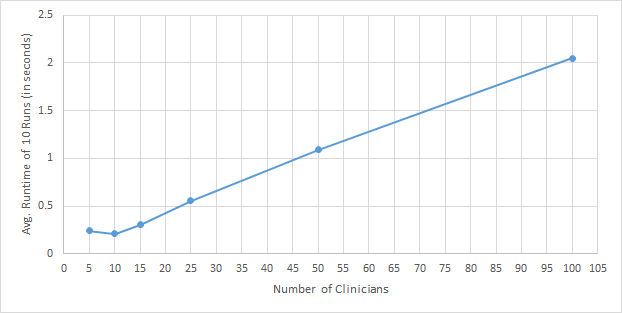
\includegraphics[scale=.6]{fig/avg_runtime_clinicians}
	\caption{Plot of average runtime for LP with an increasing number of clinicians}
	\label{fig:avg-runtime-clinicians}
\end{figure}

Next we evaluated the effect of increasing the number of departments. Figure \ref{fig:avg-runtime-divisions} shows the average runtime for a department with a 10 clinicians, and a range of divisions, $D = \{1, 2, 3\}$. We can see that increasing the number of divisions even by 2 greatly affects the runtime. The LP solver had significant trouble when we increased the number of divisions further, making it impractical to quickly generate schedules for departments with many divisions. \\

\begin{figure}[h]
	\centering
	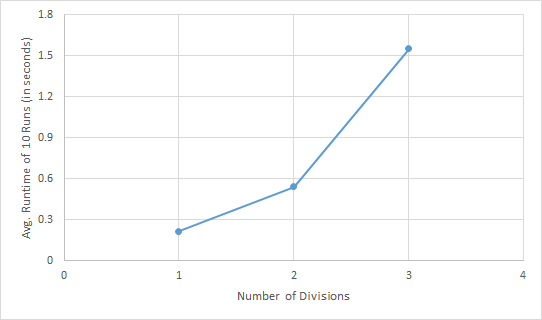
\includegraphics[scale=.6]{fig/avg_runtime_divisions}
	\caption{Plot of average runtime for LP with an increasing number of divisions}
	\label{fig:avg-runtime-divisions}
\end{figure}

We plotted the effect of an increasing number of requests per clinician on the average runtime of the LP solver in figure \ref{fig:avg-runtime-requests}. We ran the program on a single-division department with 10 clinicians, and $R = \abs{\mathcal{WR}} + \abs{\mathcal{BR}} = \{1, 2, 3, 5, 10\}$ non-overlapping requests per clinician. The increase in the number of requests did not affect the runtime of the LP solver, indicating that it can handle and accommodate much flexibility in clinician requests. \\

\begin{figure}[h]
	\centering
	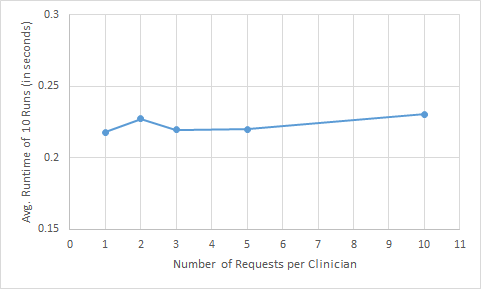
\includegraphics[scale=.6]{fig/avg_runtime_requests}
	\caption{Plot of average runtime for LP with an increasing number of requests per clinician}
	\label{fig:avg-runtime-requests}
\end{figure}

[...]
	\section{Discussion}\label{sec:discussion}
	In this paper our goal was to develop a rather simple, yet flexible, integer linear programming formulation to generate schedules for clinical departments at hospitals. The difficulty in applying such an approach to this task lies in the fact that ILP is an NP-hard problem, and as such, the time to find an optimal solution grows exponentially as we increase the size of the problem. As a result, the vast majority of approaches taken to create schedules for similar scenarios tend to use heuristics in order to find an approximately optimal solution in a shorter time. \\

Our formulation includes hard constraints to ensure the schedule satisfies hospital and logistics requirements. It also aims to satisfy the work preferences of clinicians in a clinical department by optimizing a multi-goal objective function [...] \\

We developed a tool that implements the ILP formulation and generates an optimal schedule based on provided input data. It provides a simple and easy-to-use user interface that can be used by any hospital staff to generate schedules well in advance. We compared the optimal schedule generated with the help of the tool to the manually-created schedules at St. Michael's Hospital. We found that the ILP formulation was always able to find an optimal schedule satisfying all required hard constraints, unlike the manual schedule, that often did not take all constraints into account. Moreover, due to the multi-goal objective function in the ILP, the tool was able to maximize and fulfill the majority of clinician preferences and requests, more so than the manually-created schedule. These observations reinforce the idea that it is vital to employ automated tools when generating schedules in hospital departments, to reduce human error, balance the work-load of clinicians and improve the service provided to patients. \\

We analyzed the performance of our formulation on simulated data meant to resemble real-life clinician departments at different hospitals. Our results show that increasing the number of requests per clinician does not affect the runtime of the algorithm, highlighting the flexibility of the tool in incorporating clinician preferences. Further, we saw that the algorithm can accommodate increasing the time-horizon up to four years with little impact on runtime, which can be applied to departments that generate schedules far in advance. The most notable impact on the runtime was noticed when trying to increase the number of services offered in a single department. While such cases are unlikely to be encountered in the real-world, as most departments tend to focus on a single service [ref \ref{???}], the runtime issues can be mitigated by relaxing certain constraints. \\

In future work, we can look first and foremost into improving the runtime of the tool by modifying constraints and objectives, so that it can be used in larger departments offering multiple services for their patients. On top of that, we can introduce new objectives that incorporate additional clinician preferences and allow for better distribution of work-load. However, since our ultimate goal is to maintain a ILP formulation, care must be taken not to overly complicate the model and risk running into additional time complexity issues.
	\section{Acknowledgements}\label{sec:acknowledgements}
	The authors are grateful to Julie Veitch for her contributions to testing and
designing the scheduling software. SM is supported by a Canadian Institutes of
Health Research New Investigator Award. DL conducted part of this project as a
Keenan Research Summer Student, Li Ka Shing Knowledge Institute, St.\ Michael's
Hospital, University of Toronto.

	\section{Funding}\label{sec:funding}
	The work was jointly funded by the Ontario Ministry of Science and Innovation Early Researcher Award Number ER17-13-043; the Division of Infectious Diseases, St. Michael’s Hospital, University of Toronto; and the University of Toronto Work Study Program.
	
	\bibliographystyle{unsrt}
	\bibliography{references}
\end{document}
